% 独自のコマンド

% ■ アブストラクト
%	\begin{jabstract} 〜 \end{jabstract}	:日本語のアブストラクト
%	\begin{eabstract} 〜 \end{eabstract}	:英語のアブストラクト

% ■ 謝辞
%	\begin{acknowledgment} 〜 \end{acknowledgment}

% ■ 文献リスト
%	\begin{bib}[100] 〜 \end{bib}


\newif\ifjapanese

\japanesetrue	% 論文全体を日本語で書く(英語で書くならコメントアウト)

\ifjapanese
	\documentclass[11pt]{jreport}
	\renewcommand{\bibname}{参考文献}
	\newcommand{\acknowledgmentname}{謝辞}
\else
	\documentclass[11pt]{report}
	\newcommand{\acknowledgmentname}{Acknowledgment}
\fi
\usepackage[top=30truemm,bottom=30truemm,left=25truemm,right=25truemm]{geometry}
\usepackage{ascmac}
\usepackage{graphicx}
\usepackage{multirow}
\usepackage{ylab_thesis}
\DeclareFontShape{JY1}{mc}{m}{it}{<5> <6> <7> <8> <9> <10> sgen*min
    <10.95><12><14.4><17.28><20.74><24.88> min10 <-> min10}{}
\DeclareFontShape{JT1}{mc}{m}{it}{<5> <6> <7> <8> <9> <10> sgen*tmin
    <10.95><12><14.4><17.28><20.74><24.88> tmin10 <-> tmin10}{}
\usepackage{times}
\usepackage[stable]{footmisc}
\usepackage{otf}
\usepackage{epsf}

%\bindermode	% バインダ用余白設定

% 日本語情報(必要なら)
\jclass	{卒業論文}							% 論文種別
\jtitle		{Mashup による e-learning コンテンツ検索システムの開発}			% タイトル。改行する場合は\\を入れる
\juniv		{佐賀大学}						% 大学名
\jfaculty	{理工学部知能情報システム学科}				% 学部、学科
\jauthor	{甲斐 \UTF{F9C3}馬}						% 著者 \CID{7808}でも同字が出る
\jnumber	{08233014}						% 学籍番号
\jadvisor	{新井 康平}{教授}					% 指導教官、形式は『{名前}{肩書}』
\jchief	{渡邉 義明}{教授}					% 学科長名、形式は『{名前}{肩書}』
\jhyear	{25}								% 平成○年
\jhyeared {24}								% 平成○年「度」
\jsyear	{2013}						% 西暦○年
\jsyeared	{2012}							% 西暦○年「度」
\jkeyword	{Mashup, Android, e-learning}			% 論文のキーワード

% 英語情報(必要なら)
\eclass	{Graduation Thesis}					% 論文種別
\etitle		{Development of e-learning content searcher by Mashup}	% タイトル。改行する場合は\\を入れる
\euniv	{Saga University}						% 大学名
\efaculty	{Department of Information Science, Faculty of Science and Engineering}	% 学部、学科
\eauthor	{Ryoma KAI}					% 著者
\enumber	{08233014}						% 学籍番号
\eadvisor	{Professor}{Kohei ARAI}				% 指導教官、形式は『{肩書}{名前}』
\echief		{Professor}{Yoshiaki WATANABE}				% 学科長名、形式は『{肩書}{名前}』
\eyear	{2013}							% 西暦○年
\ekeyword	{Mashup, Android, e-learning}		% 論文のキーワード



\begin{document}

\jmaketitle		% 表紙(日本語)、不要ならコメントアウト
\emaketitle		% 表紙(英語\ref{chap:latex})、不要ならコメントアウト

% ■ 概要の出力 ■
%		begin{jabstract}〜end{jabstract}	:日本語の概要
%		begin{eabstract}〜end{eabstract}	:英語の概要
%		※ 不要ならばコマンドごと消せば出力されない。

% 日本語の概要
\begin{jabstract}
近年、iOSやAndroidなどのタブレット端末・スマートフォン端末の普及が進み、それらの教育目的での利用価値も俄然高く評価されてきている。しかし、教育方面での利用のためのGUIは未だに未熟、またはなかなか考慮されにくいのが現状であり、タブレット端末での効果的な学習を支援するサービスを作ることは非常に意義深いことであると考える。本研究では、タブレット端末におけるe-learning検索アプリを、mashupと呼ばれる開発手法を用いて柔軟に開発した後、検証を行ったものである。
\end{jabstract}

% 英語の概要
\begin{eabstract}
Tablet and Smartphone (e.g. iOS and Android ) devices today has a fairly, those app's value is appreciated in educational field(e.g. e-learning). However, those app's GUI is inexperienced and not considered carefully. Therefore, it is meaningful to build educational support service. This reseach is development and veritificcation of e-learning search app with mashup in Android.
\end{eabstract}	% アブストラクト。要独自コマンド、include先参照のこと

\tableofcontents	% 目次
 \listoffigures		% 図目次、不要ならコメントアウト
% \listoftables		% 表目次、不要ならコメントアウト

\pagenumbering{arabic}

\chapter{序論}
\label{chap:introduction}

本章では、本研究の背景、それを踏まえた上での研究の目標・目的、そして文書の構成について述べる。

\section{背景}

2007年、iOS、Android OSの両オペレーティング・システムを搭載したタブレット端末やスマートフォン端末が発表された。
これら端末はスペック的にそれほど高くものではないものの、タッチパネルの搭載による直感的な操作、携帯性の高さ、Wi-fi接続によるインターネット接続が可能といった多数のメリットを兼ね備えており、欧米を中心に今日まで爆発的に普及してきている。\footnote{株式会社シード・プランニングの行った2012年7月の市場調査\cite{smartphoneresearch}によると、日本でのスマートフォン普及率は40\%前後と先進国の中ではやや低調である。元々高品質な携帯電話が普及しており、プラットフォームが盤石であったことが要因であると考えられている。}\\
一方、e-learningとは、パーソナルコンピュータなどの情報機器を用いて行う学習のことである。1990年代後半からのPCの普及と共に様々な分野で用いられるようになり、現在ではe-learningのコンテンツ共有を目的とした規格\cite{scorm}や大学設置基準に基づく文部科学省告示の中にe-learningに関する項目が記述される\cite{monkasho}など、制度や規格も整備されたものとなっている。\\
e-learningサイトの多くは、その基盤がタブレット端末、スマートフォン端末が発表されるより前に発表されたものであり、

iTunes U


\section{本文書の構成}

第1章の最後は、文書全体の構成を大まかに書くとよいらしい。

第\ref{chap:introduction}章では本テンプレートの概要みたいなものを書いた。第\ref{chap:howto}章では、本テンプレートの使い方を説明する。第\ref{chap:latex}章で図表や数式の挿入など代表的な\LaTeX コマンドを解説する。第\ref{chap:conclusion}章では、『序論』で始めたら『結論』で終われと書いた手前書かざるを得ないので、なにか結論らしいことを書く。付録として、テンプレートのサンプルになるように無理矢理ゴミを添付する。	% 序論
\chapter{MashupとWebAPI}
\label{chap:webapi}
本章では、表題となっているMashupと呼ばれる開発手法に加え、WebAPIと呼ばれるタイプのAPIについて解説する。
\section{Mashupとは}
Mashupとは、2つ以上のWebAPIを組み合わせて1つのWebサービスやアプリケーションを構成する手法のことである。元来、利用価値の高いWebサービスを作るためには、独自に検索エンジンや結果応答用のサーバを構築する必要があり、目的のWebサービスを作るために多大な労力を払う必要があった。しかし、Mashupでは、既存のデータベースを有するWebサービスから得られた応答結果を自由に組み合わせることにより、短期間で価値の高いWebサービスを製作することができる。
\section{WebAPIとは}
WebAPIとは、インターネットを介して利用することのできるアプリケーション・プログラミング・インターフェイス(API)のことである。殆どのWebAPIが一般的なURLの形式を取っており、HTTPによるPOSTメソッドを用いて、パラメータを付加したURLを使用してアクセスしてデータを取得する。返ってくるデータはXML、JSONのどちらかが一般的である。今回用いるWebAPIは、以下の4つである。
\subsection[Yahoo!検索Web API-ウェブ検索API]{Yahoo!検索Web API-ウェブ検索API\protect\footnote{ウェブ検索APIは、2013年3月頃を目処にAPIのリクエストURLが変更される予定であり、これはそれまで公開されていたアップグレード版ウェブ検索APIを使用している。}}
%\begin{table}[htdp]
\begin{tabular}{c|l}
開発 & ヤフー株式会社 \\
URL & http://search.yahooapis.jp/PremiumWebSearchService/V1/webSearch \\
機能 & Web上に公開されているページを検索する
\end{tabular}
%\end{table}
\subsection[Yahoo!検索Web API-画像検索API]{Yahoo!検索Web API-画像検索API\protect\footnote{画像検索APIは、2013年3月頃を目処にAPIのリクエストURLが変更される予定であり、これはそれまで公開されていたアップグレード版画像検索APIを使用している。}}
%\begin{table}[htdp]
\begin{tabular}{c|l}
開発 & ヤフー株式会社 \\
URL & http://search.yahooapis.jp/PremiumImageSearchService/V1/imageSearch \\
機能 & Web上に公開されている画像を検索する
\end{tabular}
%\end{table}
\subsection{Youtube Data API}
%\begin{table}[htdp]
\begin{tabular}{c|l}
開発 & Google Inc. \\
URL & http://gdata.youtube.com/feeds/api/videos \\
機能 & Youtubeの機能(動画の検索、アップロード、再生リストの作成など)を利用する
\end{tabular}
%\end{table}
\subsection{Product Advertising API}
%\begin{table}[htdp]
\begin{tabular}{c|l}
開発 & Amazon.com, Inc.\\
URL & http://ecs.amazonaws.jp/onca/xml \\
機能 & Amazon の商品情報や関連コンテンツを検索する
\end{tabular}
%\end{table}	% WebAPIについて
\chapter{検索エンジンの精度向上}
\label{chap:search}

この章では、よく使う\LaTeX のコマンドを説明する。足りない部分はぐぐればだいたいわかると思う。最初に書いておくと、数式を書く方法は、ぼく自身使わなかったので書いていない。ぼくのいた研究室でごりごり数式をたくさん書く必要のあるひとは、研究の種類からするとあまり居ない気がする。

\section{先行研究}

\subsection{e-learningコンテンツにおけるドキュメントサーチの最適化}


\section{補助キーワード}

\subsection{選出過程}

\subsection{選出結果}


	% 検索エンジンの精度向上
\chapter{WWW視覚化}
\label{chap:visualize}

この章では、WWW視覚化という目線での先行研究や開発事例、そして解決方法についての案を提起する。

\section{開発事例}
この分野における開発事例や先行研究は多数存在しているが、中でも3次元CGによる視覚化を実現しているUNIXソフトウェア「納豆ビュー\cite{natto}」と、mashupによる検索エンジンのWWW視覚化を実現しているWebサービス「Flowser\cite{flowser}」について解説する。

\subsection{納豆ビュー}
\begin{figure}[htbp]
\begin{center}
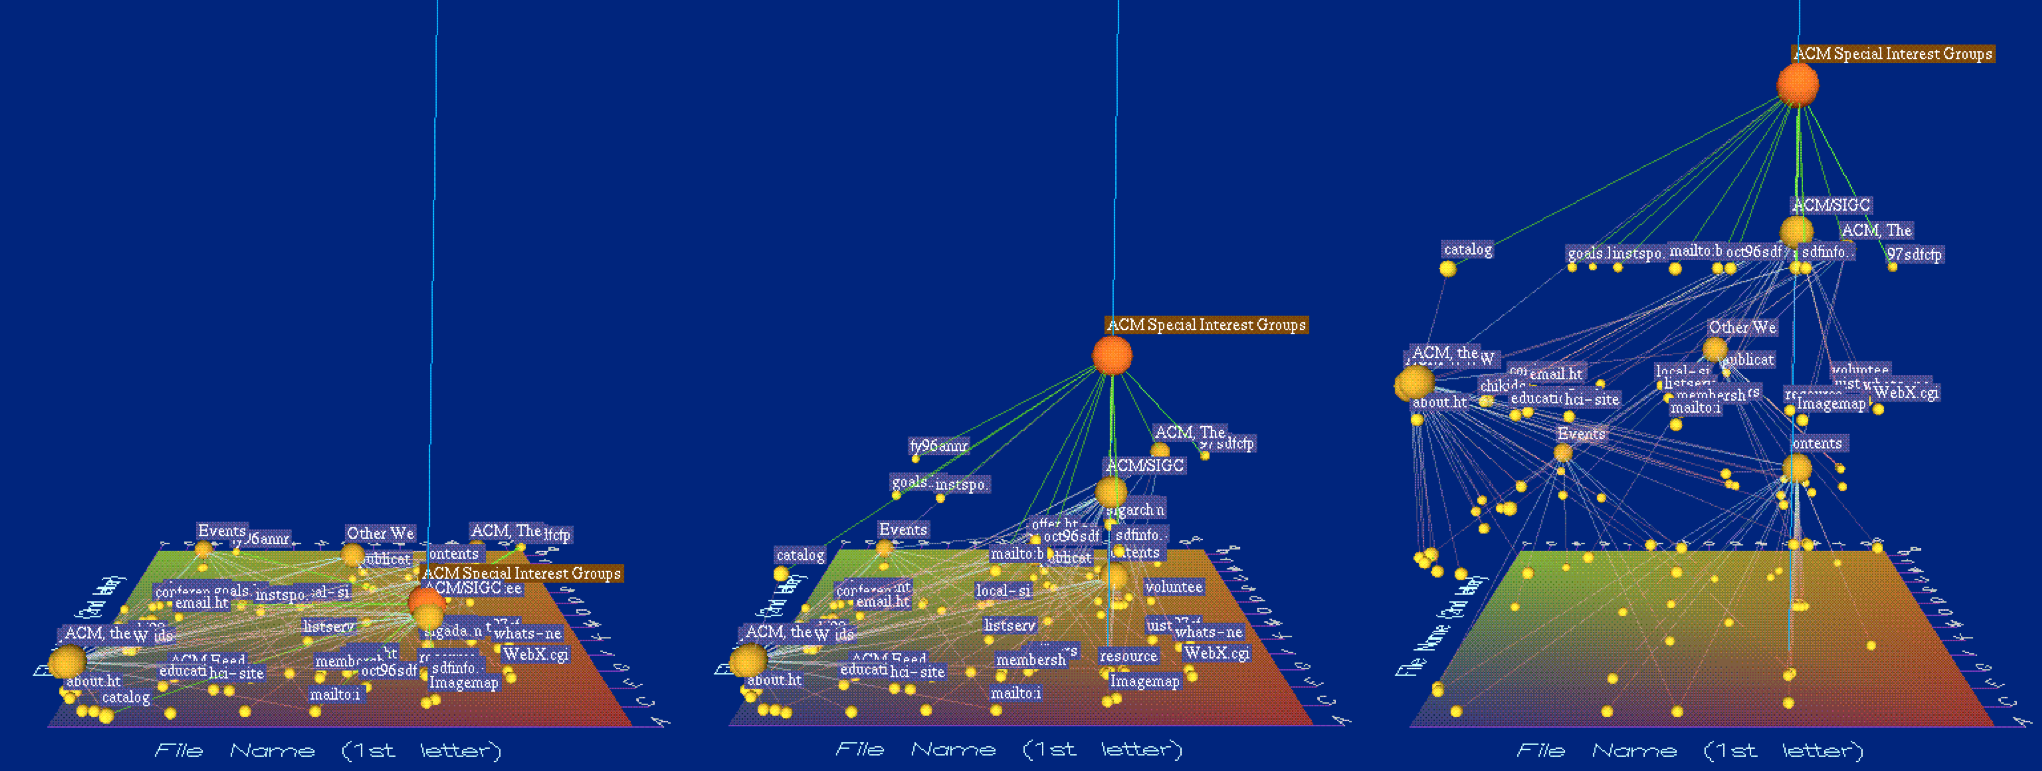
\includegraphics[width=15cm]{natto.eps}
\caption{納豆ビュー}
\label{納豆ビュー}
\end{center}
\end{figure}
UNIXのX-Window System、Mesa、GLUTを用いており、3次元CGグラフ上に展開したノードをリンクに見立て、リンク・被リンクにある関係がエッジで表示される。xy平面には一意的な座標が与えられ、z軸方向にはノードを摘んで持ち上げる、つまりユーザによる操作が可能となっている。これにより、複雑なネットワークをユーザーの意志によってわかりやすく可視化できるようになっている。

\subsection{Flowser}
\begin{figure}[htbp]
\begin{center}
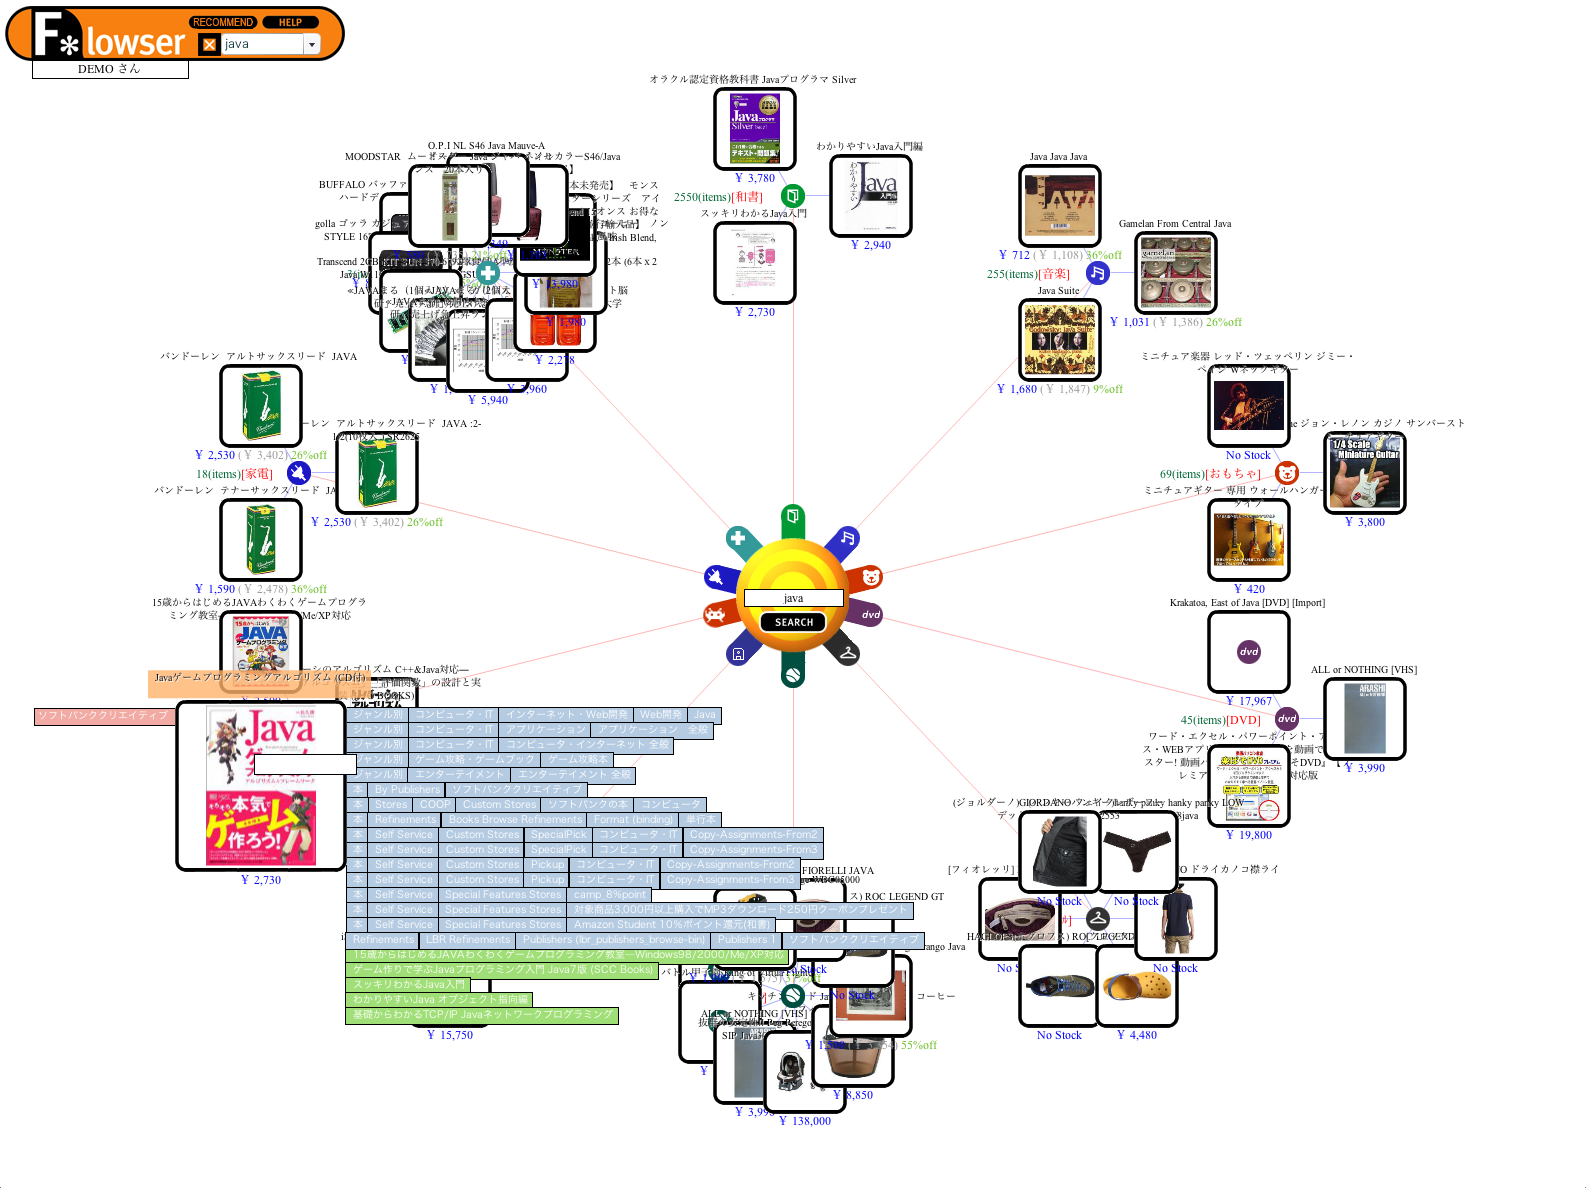
\includegraphics[width=15cm]{flowser.eps}
\caption{Flowser}
\label{flowser}
\end{center}
\end{figure}
Product Advertising APIを用いたWebサービスであり、Mashupの作例でもある。検索ボックスに入力したキーワードからAmazonの複数ジャンルの商品を一気に検索・閲覧することができ、通常のサイトを通じた検索では得られなかった情報を届けることを可能にした。

\section{検索エンジンにおけるWWW視覚化}
以上2つの開発事例を見たところで、改めて、今回の研究で解決したい問題を整理する。
\begin{itemize}
\item タブレットやスマートフォン上から検索結果への直感的な操作
\\
直感的に結果を閲覧するためには、納豆ビューのようにユーザー自身によって結果をわかりやすく可視化できるようにする工夫が必要になる。また、タブレットやスマートフォンでの閲覧を前提とするため、画面サイズやボタンサイズなど、操作性に対する配慮も必要となる。
\\
\item 複数のコンテンツ(検索エンジン)を同時に検索
\\
e-learningコンテンツは、Webページだけでなく、動画、画像、PDFなどの文書ファイルのように、多数の形式に分かれていることが考えられる。であれば、Flowser.comのように、複数結果をそれぞれ分離して見やすく表示する必要がある。
\\
\item e-learningコンテンツへの導線
\\
コンテンツを検索して終了、ではなく、検索したコンテンツへはダイレクトにアクセス可能にする。ページであればブラウザでの表示を行い、動画であればタップと同時に動画サイトやアプリへ遷移し、再生を開始する必要がある。
\end{itemize}

以上の条件から、4つの表示モデルを考えた。

\subsection{Helixモデル}
\begin{figure}[htbp]
\begin{center}
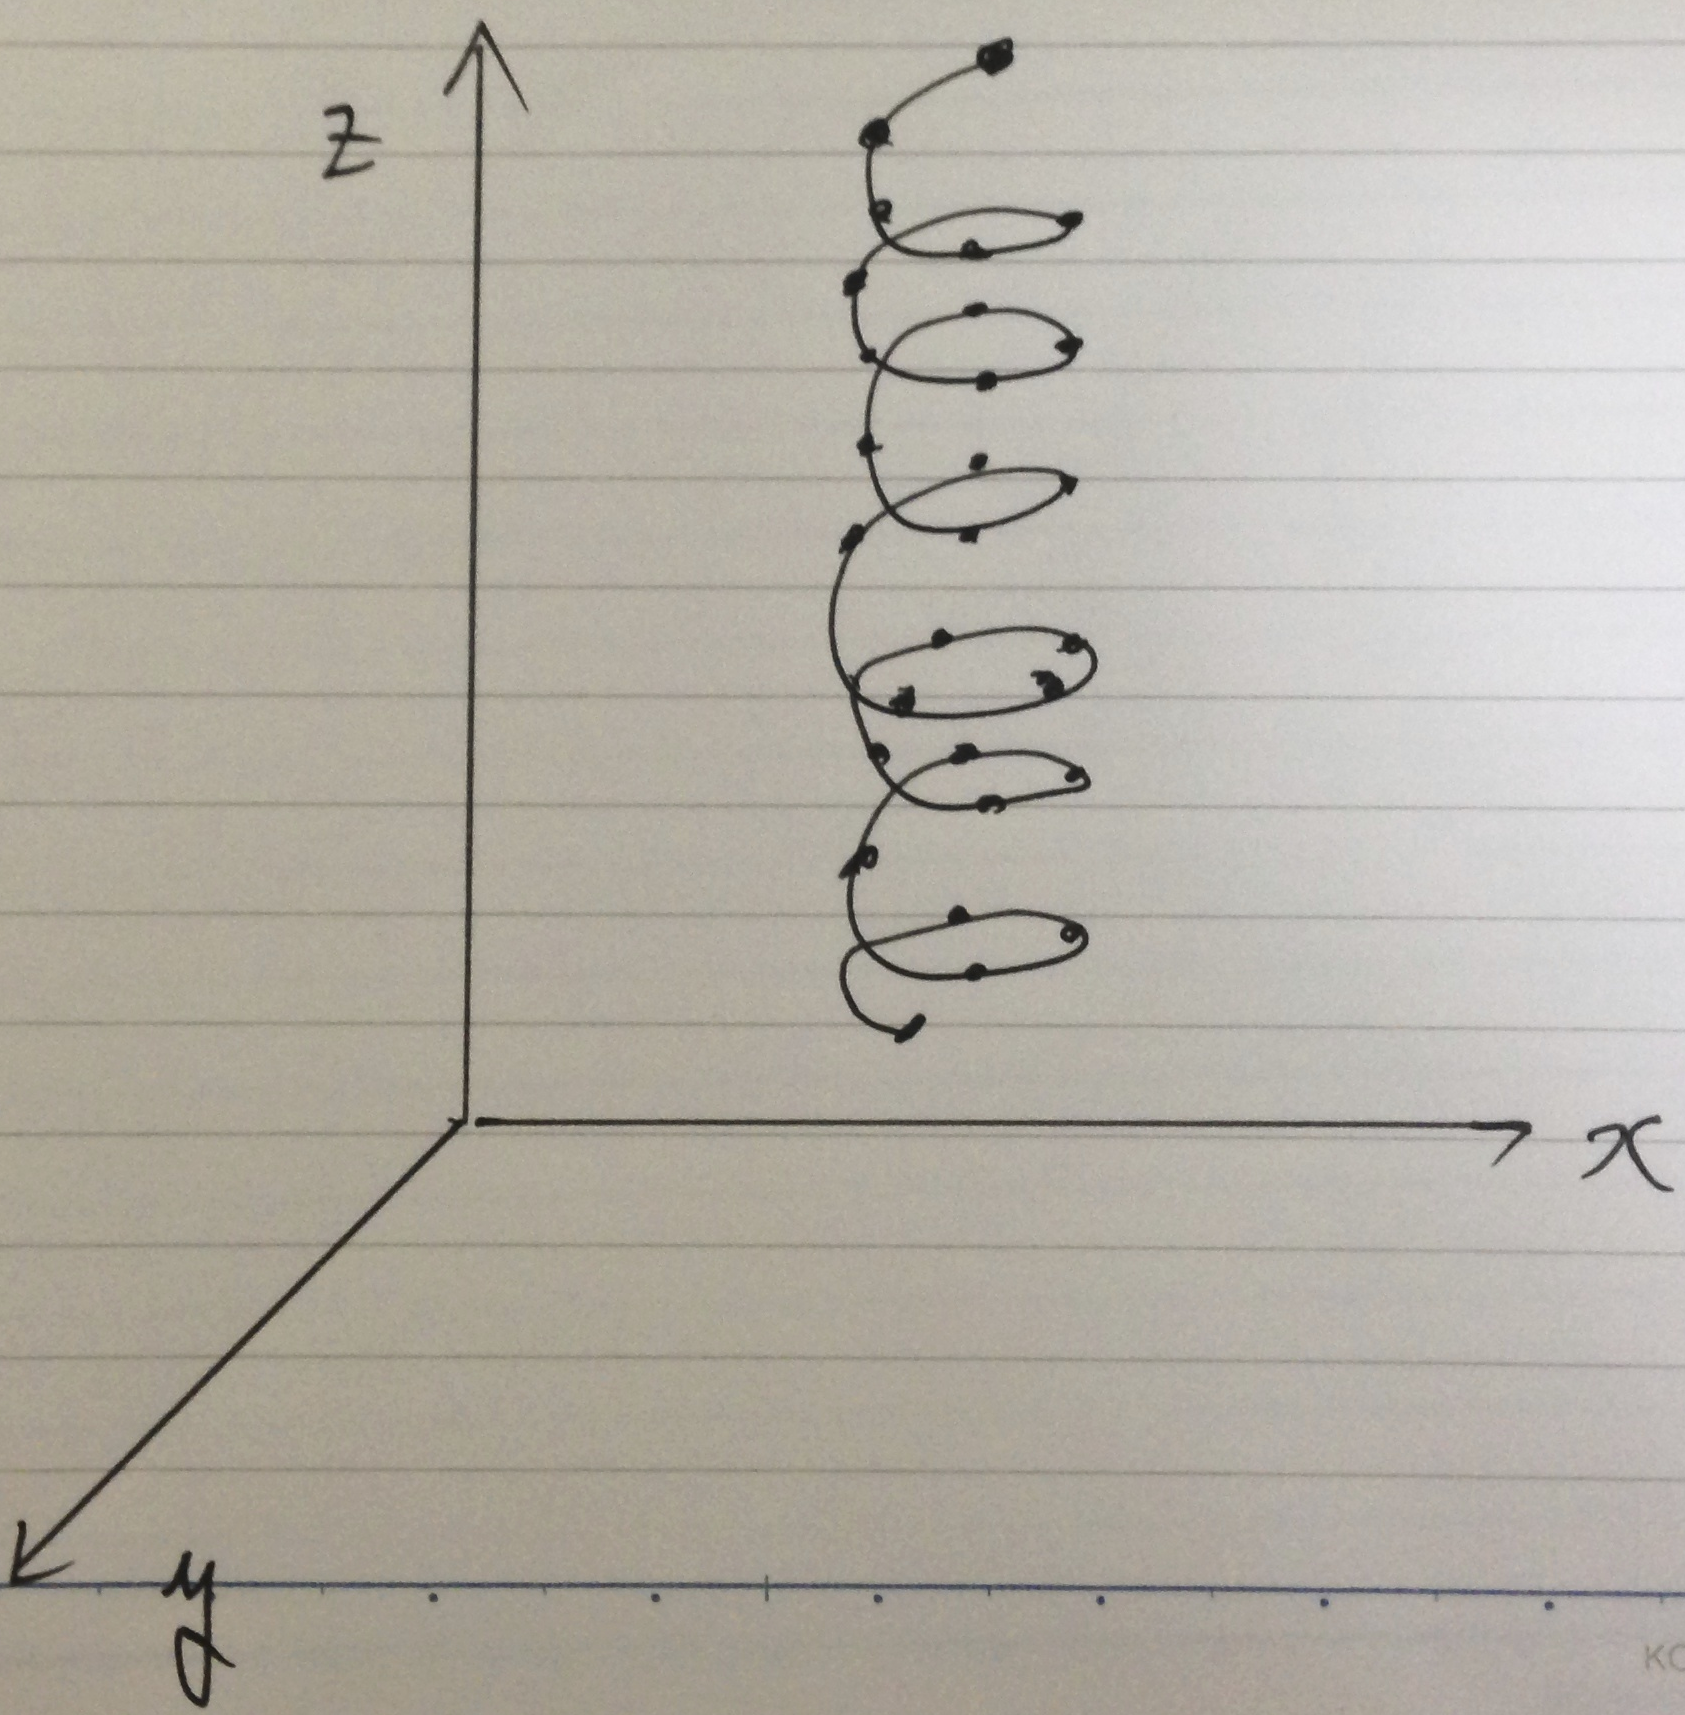
\includegraphics[width=15cm]{helix.eps}
\caption{Helixモデル}
\label{helix}
\end{center}
\end{figure}
3次元螺旋の円周上に検索結果のコンテンツを配置し、螺旋階段を降りるように検索結果の下位コンテンツへと閲覧していくモデルである。この方法の優れた点として、螺旋階段の中心線からコンテンツを見た時、コンテンツ同士の下位と上位が判断しやすく、ユーザがどのような方向にスワイプしても検索結果を辿れる、つまり上下左右方向への持ち替えが容易であるといった利点がある。しかし、複数コンテンツへの対応を考えた際、螺旋一つでは画面上に対しての情報量に無駄が多く、複数コンテンツへ対応しきれない可能性が高いと考えられる。

\subsection{Starモデル}
\begin{figure}[htbp]
\begin{center}
\includegraphics[width=15cm]{star.eps}
\caption{Starモデル}
\label{star}
\end{center}
\end{figure}
複数コンテンツへの配置を最優先に考え、Flowser.comのような円形状のコンテンツ展開を考えたモデルである。コンテンツ毎にそれぞれのノードに分類され、そこから3次元上にランダムにノードが生えており、このノードまでのエッジの長さが検索結果の上位と下位を表している。しかし、3次元上に無作為にノードが存在しているため、コンテンツの一覧性には著しく欠けており、視点を定め辛いことが考えられる。

\subsection{Star-Helixモデル}
\begin{figure}[htbp]
\begin{center}
\includegraphics[width=15cm]{star-helix.eps}
\caption{Star-Helixモデル}
\label{star-helix}
\end{center}
\end{figure}
Helix modelとStar model、両者のメリットをうまく併せて設計したモデルである。螺旋はコンテンツジャンルの数だけ存在し、円形状に展開した始点から同方向に対して一様に伸びている。しかし、複数の螺旋を同時に見れる視点の位置が一意に決まらないため、ユーザーが混乱する可能性が高い。

\subsection{Star-Slideモデル}
\begin{figure}[htbp]
\begin{center}
\includegraphics[width=15cm]{star-line.eps}
\caption{Star-Slideモデル}
\label{star-line}
\end{center}
\end{figure}
Star modelのコンテンツ分離性を活かし、そこから垂直、同方向にコンテンツを配置したモデルである。このモデルを外周から見ると、ちょうど画面上にすべてのコンテンツが入るようになっており、非常に視認性に優れている。加えて、スワイプによって移動する方向も一意であることから、ユーザーが混乱しにくい。また、最前方に配置するコンテンツは丸型ハンガーラックのように回転するようになっており、別のコンテンツをメインに見たい、という時には横方向へのスワイプで自由に切り替えられるようになっている。

\section{採用手法}
以上より、最も多くの問題を改善できた方法として、Star-Slide modelの採用を決定した。	% WWW視覚化
\chapter{開発手法}
\label{chap:coding}

本章では、本研究の背景、それを踏まえた上での研究の目標・目的、そして文書の構成について述べる。

\section{概観}


\section{Away3D}

\subsection{Away3Dとは}

\subsection{Android上への移植}


	% 開発手法
\chapter{Androidアプリ「LEDOXEA」}
\label{chap:ledoxea}

本章では、開発したAndroidアプリ「LEDOXEA」の利用方法と、その特徴について説明する。

\section{使用方法}
起動後、上部にある検索ボックスから、検索したいキーワードを入力する。入力が完了したら、右側の検索ボタンを押下する。すると検索が行われ、合計5本のラインが画面上に出現する。これらを上下にスワイプすると、検索結果の上下移動が可能であり、ひとつひとつ項目を参照することが可能である。また、別のコンテンツを参照したい時は、左右にスワイプすると回転ハンガーのようにコンテンツが回転し、別のコンテンツが中央に移動する。

\section{特徴}
それぞれ実現することができた、特徴について記述する。

\subsection{移植性}
ADOBE AIR の移植性の高さにより、Androidに留まらず、iOS、PCのWebブラウザ、PCアプリケーションとして様々な形態に対応できる。

\subsection{スペック性能への非依存性}
非常に簡易な3次元CGにより製作されているため、60fps程度の安定した高速描画を実現している。

\subsection{フリック操作による直感的操作性}
検索結果を上下や左右に移動するのは直感的に理解しやすく、項目を確認する際に発生する苦痛を軽減することに役立つ。

\subsection{検索エンジンの同時検索、WWW視覚化}
e-learningコンテンツを複数の検索エンジンで同時に高精度で検索できるため、一度の検索で非常に多量の収穫を得ることをできる。	% Androidアプリ「LEDOXEA」
\chapter{アンケートによる評価と考察}
\label{chap:result}

本章では、本研究の背景、それを踏まえた上での研究の目標・目的、そして文書の構成について述べる。

\section{評価結果}


\section{考察}


	% アンケートによる評価と考察
\chapter{結論}
\label{chap:conclusion}

この章では、結論らしいことをかく。


	% まとめ


\begin{acknowledgment}
本研究を卒業論文として完成させることができたのは、担当して頂いた新井康平教授、Herman Tolle博士研究員の熱心なご指導や、第4研究グループの皆様方に協力して頂いたおかげです。皆様へ心より感謝の気持ちと御礼を申し上げたく、謝辞に代えさせていただきます。
\end{acknowledgment}
	% 謝辞。要独自コマンド、include先参照のこと
\begin{bib}[100]


% \bibitem{参照用名称}
%   著者名: 
%   \newblock 文献名,
%   \newblock 書誌情報,出版年.


\bibitem{smartphoneresearch}
\begin{flushleft}
  株式会社シートプランニング:
  \newblock 世界のスマートフォン普及予測
  \newblock {\it http://www.seedplanning.co.jp/press/2012/2012072601.html}, 2012.7.26.
\end{flushleft}

\bibitem{scorm}
\begin{flushleft}
  Advenced Distributed Learning(ADL):
  \newblock SCORM,
  \newblock {\it http://www.adlnet.gov/capabilities/scorm}, 2004.
\end{flushleft}
  
\bibitem{itunesu}
\begin{flushleft}
  Apple,Inc.:
  \newblock iTunes U,
  \newblock {\it http://www.apple.com/jp/education/itunes-u/}, 2004. 
\end{flushleft}

\bibitem{monkasho}
\begin{flushleft}
  文部科学省:
  \newblock 平成十三年文部科学省告示第五十一号(大学設置基準第二十五条第二項の規定に基づく大学が履修させることができる授業等),
  \newblock {\it http://www.mext.go.jp/b\_menu/hakusho/nc/k20010330001/k20010330001.html}, 2001.
\end{flushleft}

\bibitem{docsearch}
\begin{flushleft}
  原真琴:
  \newblock e-learningコンテンツにおけるドキュメントサーチの最適化,
  \newblock 2012.3.
\end{flushleft}

\bibitem{natto}
\begin{flushleft}
  塩澤秀和, 西山晴彦, 松下温:
  \newblock 「納豆ビュー」の対話的 な情報視覚化における位置づけ,
  \newblock 情報処理学会論文誌 Vol.38 No.11, pp.2331-2342, 1997.11.
\end{flushleft}

\bibitem{flowser}
\begin{flushleft}
  有限会社ジャックポット:
  \newblock Flowser,
  \newblock {\it http://flowser.com/}, 2005.4.
\end{flushleft}

\bibitem{away3d}
\begin{flushleft}
  Away3D Team:
  \newblock Away3D,
  \newblock {\it http://away3d.com/}, 2007.
\end{flushleft}

\bibitem{bulkloader}
\begin{flushleft}
  Arthur Debert:
  \newblock Bulk Loader,
  \newblock {\it http://github.com/arthur-debert/BulkLoader}, 2010.
\end{flushleft}

\bibitem{as3crypto}
\begin{flushleft}
  Henri Torgemane:
  \newblock As3 Crypto,
  \newblock {\it http://code.google.com/p/as3crypto/}, 2008.6.
\end{flushleft}

\end{bib}	% 参考文献。要独自コマンド、include先参照のこと
\appendix
\chapter{プログラム}
実装したActionScriptのソースコード、並びにAndroidアプリを定義するxmlファイルを掲載する。実装はFlashCS6を用いて、Android2.2端末(IS04)での動作を確認している。

\section{main.as(ActionScript)}
\begin{itembox}[l]{{未完成}}
\begin{verbatim}
ギリギリまで粘ったものを添付する予定です……
\end{verbatim}
\end{itembox}

\section{app.xml(XML)}
{\scriptsize
\begin{verbatim}
<?xml version="1.0" encoding="utf-8" standalone="yes"?>
<application xmlns="http://ns.adobe.com/air/application/3.2">
  <id>legdoxea</id>
  <versionNumber>1.0.0</versionNumber>
  <filename>Legdoxea</filename>
  <description>3D view e-learning searcher</description>
  <name>Legdoxea</name>
  <copyright></copyright>
  <initialWindow>
    <content>Legdoxea.swf</content>
    <systemChrome>standard</systemChrome>
    <transparent>false</transparent>
    <visible>true</visible>
    <fullScreen>true</fullScreen>
    <autoOrients>false</autoOrients>
    <aspectRatio>portrait</aspectRatio>
    <renderMode>direct</renderMode>
    <depthAndStencil>true</depthAndStencil>
  </initialWindow>
  <customUpdateUI>false</customUpdateUI>
  <allowBrowserInvocation>false</allowBrowserInvocation>
  <icon></icon>
  <android>
    <manifestAdditions><![CDATA[<manifest>
      <uses-permission android:name="android.permission.INTERNET"/>
    </manifest>]]></manifestAdditions>
  </android>
  <versionLabel></versionLabel>
  <supportedLanguages>en ja</supportedLanguages>
</application>
\end{verbatim}
 }
		% 付録

\end{document}
